% =====================================================================
\chapter{Diferenciación numérica y comprobación de gradientes}
\label{tema:6}
% =====================================================================

Un error en la implementación de un gradiente no suele provocar un fallo visible: el entrenamiento avanza, pero peor de lo que debería. La herramienta estándar para detectarlo es comparar el gradiente analítico con una aproximación por diferencias finitas. Este tema analiza el error de truncamiento de las diferencias finitas con el teorema de Taylor, el error de redondeo de la aritmética de coma flotante y el compromiso entre ambos, y describe el procedimiento de comprobación de gradientes. Se sigue~\cite[§4.1]{gbc} y las notas de~\cite{cs231n}.

\section{Diferencias finitas}

\begin{definicion}[Diferencias finitas]\label{def:diferencias}
Sea $f\colon\R^{n}\to\R$ y $h>0$. Las \emph{diferencias hacia delante} y \emph{centrada} en la coordenada $i$ son
\[
\Delta_i^{+}f(x)=\frac{f(x+h\,e_i)-f(x)}{h},\qquad
\Delta_i^{c}f(x)=\frac{f(x+h\,e_i)-f(x-h\,e_i)}{2h}.
\]
Ambas aproximan $\partial f/\partial x_i(x)$ cuando $h\to 0$.
\end{definicion}

\begin{proposicion}[Error de truncamiento]\label{prop:truncamiento}
Sea $\phi\colon\R\to\R$ y $x\in\R$.
\begin{enumerate}
  \item Si $\phi\in C^{2}$, existe $\xi\in(x,x+h)$ tal que $\dfrac{\phi(x+h)-\phi(x)}{h}=\phi'(x)+\dfrac{h}{2}\,\phi''(\xi)$.
  \item Si $\phi\in C^{3}$, existe $\xi\in(x-h,x+h)$ tal que $\dfrac{\phi(x+h)-\phi(x-h)}{2h}=\phi'(x)+\dfrac{h^{2}}{6}\,\phi'''(\xi)$.
\end{enumerate}
En consecuencia, el error de la diferencia hacia delante es $O(h)$ y el de la centrada es $O(h^{2})$.
\end{proposicion}

\begin{proof}
(i) Es el teorema de Taylor con resto de Lagrange de orden~2: $\phi(x+h)=\phi(x)+h\phi'(x)+\tfrac{h^{2}}{2}\phi''(\xi)$; basta restar $\phi(x)$ y dividir por $h$.

(ii) Con resto de orden~3, $\phi(x\pm h)=\phi(x)\pm h\phi'(x)+\tfrac{h^{2}}{2}\phi''(x)\pm\tfrac{h^{3}}{6}\phi'''(\xi_\pm)$, con $\xi_+\in(x,x+h)$ y $\xi_-\in(x-h,x)$. Al restar, los términos de orden par se cancelan:
\[
\frac{\phi(x+h)-\phi(x-h)}{2h}=\phi'(x)+\frac{h^{2}}{6}\cdot\frac{\phi'''(\xi_+)+\phi'''(\xi_-)}{2}.
\]
La media de los dos valores de $\phi'''$ está entre ambos y, por el teorema de los valores intermedios aplicado a la función continua $\phi'''$, es igual a $\phi'''(\xi)$ para algún $\xi\in(x-h,x+h)$.
\end{proof}

Para una función de varias variables se aplica la proposición a $\phi(t)=f(x+t\,e_i)$.

\begin{ejemplo}\label{ej:exp}
Para $f(x)=e^{x}$ en $x=0$, con derivada exacta~1, la \cref{prop:truncamiento} predice errores de $h/2$ y $h^{2}/6$ aproximadamente. El \cref{tab:exp} lo confirma: al dividir $h$ entre~10, el error hacia delante se divide entre~10 y el centrado entre~100.
\end{ejemplo}

\begin{table}[h]
\centering\small
\caption{Diferencias finitas para $f(x)=e^{x}$ en $x=0$ (\cref{ej:exp}).}\label{tab:exp}
\begin{tabular}{@{}lllll@{}}
\toprule
$h$ & Hacia delante & Error & Centrada & Error \\
\midrule
$0{,}1$ & $1{,}051709$ & $5{,}17\cdot 10^{-2}$ & $1{,}001668$ & $1{,}67\cdot 10^{-3}$ \\
$0{,}01$ & $1{,}005017$ & $5{,}02\cdot 10^{-3}$ & $1{,}0000167$ & $1{,}67\cdot 10^{-5}$ \\
$0{,}001$ & $1{,}000500$ & $5{,}00\cdot 10^{-4}$ & $1{,}00000017$ & $1{,}67\cdot 10^{-7}$ \\
\bottomrule
\end{tabular}
\end{table}

\section{Error de redondeo y elección del paso}

En aritmética de coma flotante, cada evaluación de $f$ tiene un error relativo de redondeo del orden del \emph{épsilon de la máquina} $\varepsilon_{\text{máq}}$: unos $1{,}1\cdot 10^{-16}$ en doble precisión (fp64), $6{,}0\cdot 10^{-8}$ en simple precisión (fp32) y $3{,}9\cdot 10^{-3}$ en el formato bf16 que se usa para entrenar modelos de lenguaje~\cite[§4.1]{gbc}. Al restar dos valores casi iguales, $f(x+h)$ y $f(x-h)$, los errores absolutos, de tamaño $\varepsilon_{\text{máq}}\abs{f(x)}$, no disminuyen, y al dividir por $2h$ se amplifican.

\begin{proposicion}[Paso óptimo de la diferencia centrada]\label{prop:h-optimo}
Supóngase que cada evaluación de $f$ tiene un error absoluto a lo sumo $\varepsilon\abs{f}$ y que $\abs{\phi'''}\le M$ cerca de $x$. Entonces el error total de la diferencia centrada está acotado por
\[
E(h)=\frac{\varepsilon\abs{f}}{h}+\frac{M h^{2}}{6},
\]
que alcanza su mínimo en
\[
h^{*}=\Bigl(\frac{3\varepsilon\abs{f}}{M}\Bigr)^{1/3},\qquad E(h^{*})=\frac{M}{2}\,(h^{*})^{2}=O\bigl(\varepsilon^{2/3}\bigr).
\]
\end{proposicion}

\begin{proof}
El numerador calculado difiere del exacto en a lo sumo $2\varepsilon\abs{f}$, y al dividir por $2h$ se obtiene el primer término; el segundo es la cota de truncamiento de la \cref{prop:truncamiento}(ii). En $(0,\infty)$, $E'(h)=-\varepsilon\abs{f}/h^{2}+Mh/3$ se anula solo en $h^{*}$, con $E'<0$ antes y $E'>0$ después, luego $h^{*}$ es el mínimo. Sustituyendo $\varepsilon\abs{f}=M(h^{*})^{3}/3$ se obtiene $E(h^{*})=M(h^{*})^{2}/3+M(h^{*})^{2}/6=M(h^{*})^{2}/2$.
\end{proof}

Con $\abs{f}\approx M\approx 1$ y doble precisión, $h^{*}\approx(3{,}3\cdot 10^{-16})^{1/3}\approx 7\cdot 10^{-6}$ y el error mínimo es del orden de $10^{-11}$. Pasos más pequeños empeoran el resultado (\cref{fig:error-h}). En simple precisión, $h^{*}\approx 6\cdot 10^{-3}$ y el error mínimo es del orden de $10^{-5}$; en bf16 la comprobación carece de sentido. Por ello, los gradientes se comprueban siempre en doble precisión.

\begin{figure}[h]
\centering
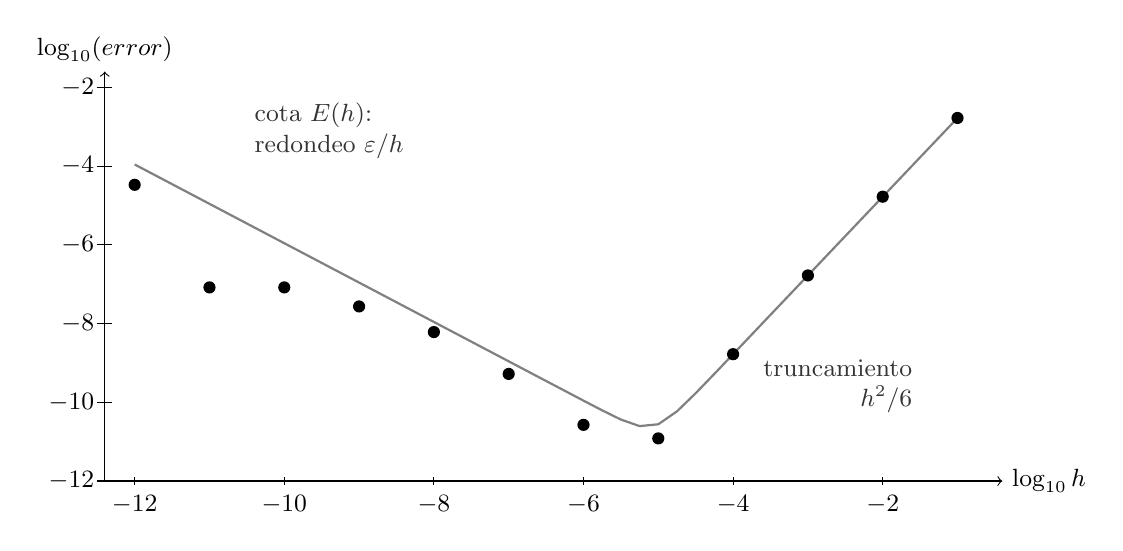
\begin{tikzpicture}[x=0.95cm,y=0.5cm,font=\small]
  \draw[->] (-12.4,-12) -- (-0.4,-12) node[right] {$\log_{10}h$};
  \draw[->] (-12.4,-12) -- (-12.4,-1.6) node[above] {$\log_{10}(\text{error})$};
  \foreach \t in {-12,-10,-8,-6,-4,-2} {\draw (\t,-12.1) -- (\t,-11.9) node[below=3pt] {$\t$};}
  \foreach \e in {-12,-10,-8,-6,-4,-2} {\draw (-12.5,\e) -- (-12.3,\e) node[left=3pt] {$\e$};}
  \draw[thick,gray] plot coordinates {(-12.00,-3.959) (-11.75,-4.209) (-11.50,-4.459) (-11.25,-4.709) (-11.00,-4.959) (-10.75,-5.209) (-10.50,-5.459) (-10.25,-5.709) (-10.00,-5.959) (-9.75,-6.209) (-9.50,-6.459) (-9.25,-6.709) (-9.00,-6.959) (-8.75,-7.209) (-8.50,-7.459) (-8.25,-7.709) (-8.00,-7.959) (-7.75,-8.209) (-7.50,-8.459) (-7.25,-8.709) (-7.00,-8.959) (-6.75,-9.209) (-6.50,-9.459) (-6.25,-9.708) (-6.00,-9.958) (-5.75,-10.205) (-5.50,-10.438) (-5.25,-10.605) (-5.00,-10.558) (-4.75,-10.230) (-4.50,-9.769) (-4.25,-9.277) (-4.00,-8.778) (-3.75,-8.278) (-3.50,-7.778) (-3.25,-7.278) (-3.00,-6.778) (-2.75,-6.278) (-2.50,-5.778) (-2.25,-5.278) (-2.00,-4.778) (-1.75,-4.278) (-1.50,-3.778) (-1.25,-3.278) (-1.00,-2.778)};
  \foreach \p in {(-1,-2.778),(-2,-4.778),(-3,-6.778),(-4,-8.778),(-5,-10.917),(-6,-10.573),(-7,-9.279),(-8,-8.216),(-9,-7.565),(-10,-7.082),(-11,-7.082),(-12,-4.476)} {\fill \p circle (2.2pt);}
  \node[gray!40!black,align=left] at (-9.4,-3.1) {cota $E(h)$:\\ redondeo $\varepsilon/h$};
  \node[gray!40!black,align=right] at (-2.6,-9.6) {truncamiento\\ $h^{2}/6$};
\end{tikzpicture}
\caption{Error de la diferencia centrada para $f(x)=e^{x}$ en $x=0$, calculada en doble precisión (puntos), y cota $E(h)$ de la \cref{prop:h-optimo} con $\varepsilon=1{,}1\cdot 10^{-16}$ y $\abs{f}=M=1$ (línea). A la derecha domina el truncamiento (pendiente~2); a la izquierda, el redondeo (pendiente~$-1$). El error medido mínimo, $1{,}2\cdot 10^{-11}$, se obtiene con $h=10^{-5}$.}
\label{fig:error-h}
\end{figure}

\section{Comprobación de gradientes}

\begin{definicion}[Error relativo]\label{def:error-relativo}
Sean $a$ una componente del gradiente analítico y $n$ la correspondiente aproximación numérica, no ambas nulas. Su \emph{error relativo} es
\[
r(a,n)=\frac{\abs{a-n}}{\max(\abs{a},\abs{n})}.
\]
\end{definicion}

El error relativo, a diferencia del absoluto, no depende de la escala del gradiente. Las notas de~\cite{cs231n} proponen como orientación, para comprobaciones en doble precisión: $r>10^{-2}$ indica casi con seguridad un error; $10^{-4}<r<10^{-2}$ es sospechoso, salvo en funciones con puntos no derivables; $r\le 10^{-7}$ indica un gradiente correcto. En redes profundas, el error relativo tiende a crecer con la profundidad.

\begin{proposicion}[Coste de la comprobación]\label{prop:coste-fd}
Calcular el gradiente completo de $f\colon\R^{N}\to\R$ por diferencias centradas requiere $2N$ evaluaciones de $f$. En cambio, para una dirección $v\in\R^{N}$, la derivada direccional $\nabla f(x)\T v$ se aproxima con dos evaluaciones:
\[
\nabla f(x)\T v=\frac{f(x+hv)-f(x-hv)}{2h}+O(h^{2}).
\]
\end{proposicion}

\begin{proof}
La primera afirmación se sigue de la \cref{def:diferencias}: dos evaluaciones por coordenada. Para la segunda, se aplica la \cref{prop:truncamiento}(ii) a $\phi(t)=f(x+tv)$, cuya derivada en $0$ es $\nabla f(x)\T v$ por el \cref{lem:curva}.
\end{proof}

La retropropagación obtiene el gradiente completo con un coste equivalente a unas pocas evaluaciones de $f$ (\cref{prop:modos}). Las diferencias finitas, por tanto, no sirven para entrenar, sino para \emph{verificar}. El procedimiento habitual es el siguiente~\cite{cs231n}:
\begin{enumerate}[label=\arabic*.]
  \item usar doble precisión y un modelo o un lote pequeños, con pocos datos;
  \item comparar componentes elegidas al azar, o derivadas direccionales en direcciones aleatorias, mediante el error relativo;
  \item tomar $h$ del orden de $10^{-5}$ y repetir con $10^{-4}$ y $10^{-6}$ si el resultado es dudoso;
  \item vigilar los puntos no derivables, como $t=0$ en ReLU: si $x-h$ y $x+h$ quedan a distintos lados de uno de ellos, la aproximación numérica no es fiable.
\end{enumerate}

\begin{observacion}[Conexión con los LLM]
Las bibliotecas de diferenciación automática incluyen utilidades de comprobación de este tipo, como \texttt{torch.autograd.gradcheck} en PyTorch, que comparan los gradientes analítico y numérico en doble precisión. Se usan al implementar una operación nueva, por ejemplo una variante de la atención, antes de emplearla en un modelo grande.
\end{observacion}

\begin{lecturas}
\item Goodfellow, Bengio y Courville~\cite{gbc}, §4.1 «Overflow and Underflow».
\item Stanford CS231n~\cite{cs231n}, notas «Neural Networks Part 3», sección «Gradient checks».
\item Deisenroth, Faisal y Ong~\cite{mml}, §5.1 (Taylor en una variable).
\end{lecturas}

\section*{Ejercicios del tema 6}
\addcontentsline{toc}{section}{Ejercicios del tema 6}

\begin{ejercicio}{1}{eje:6-porque}
¿Por qué no se entrena un LLM calculando el gradiente por diferencias finitas, si son tan sencillas de implementar? ¿Para qué se usan entonces?
\end{ejercicio}

\begin{ejercicio}{2}{eje:6-cubo}
Para $f(x)=x^{3}$ en $x=1$, calcule la diferencia hacia delante y la centrada con $h=0{,}1$ y $h=0{,}01$. ¿Cómo disminuye cada error al dividir $h$ entre~10? Compare con la \cref{prop:truncamiento}.
\end{ejercicio}

\begin{ejercicio}{2}{eje:6-direccional}
Sea $f(x,y)=x^{2}y+3y$. Compruebe el gradiente $\nabla f(2,1)=(4,7)\T$ en la dirección $v=(1,1)\T$ mediante la \cref{prop:coste-fd} con $h=0{,}01$, y calcule el error relativo.
\end{ejercicio}

\begin{ejercicio}{2}{eje:6-cs231n}
Una comprobación de gradientes en doble precisión da los siguientes pares (analítico, numérico): (a) $(1;\,1{,}0000001)$; (b) $(0{,}5;\,0{,}52)$; (c) $(10^{-3};\,1{,}0005\cdot 10^{-3})$. Calcule el error relativo de cada par y valore el resultado. (d) Para $f(x)=\max(0,x)$ en $x=10^{-6}$ con $h=10^{-5}$, calcule la diferencia centrada y su error relativo respecto de la derivada exacta, y explique el resultado.
\fuente{adaptado de Stanford CS231n~\cite{cs231n}, notas «Neural Networks Part 3», sección «Gradient checks» (criterios de error relativo y puntos no derivables).}
\end{ejercicio}

\begin{ejercicio}{2}{eje:6-fermi}
Se desea comprobar por diferencias centradas el gradiente completo de un modelo de $7\cdot 10^{9}$ parámetros. ¿Cuántas evaluaciones de la pérdida se necesitan? Si cada una tarda 1~s, ¿cuántos años se tardaría? ¿Qué se haría en su lugar?
\end{ejercicio}

\begin{ejercicio}{3}{eje:6-hoptimo}
Demuestre la \cref{prop:h-optimo} con todo detalle. Calcule $h^{*}$ y $E(h^{*})$ para $f(x)=e^{x}$ en $x=0$ con $\varepsilon=1{,}1\cdot 10^{-16}$ y compárelos con la \cref{fig:error-h}. Repita el razonamiento para la diferencia hacia delante y demuestre que, en ese caso, el paso óptimo es de orden $\varepsilon^{1/2}$ y el error mínimo también.
\end{ejercicio}
